% arara: lualatex
\documentclass{standalone}
\usepackage{mathtools}
\usepackage{unicode-math}
\unimathsetup{math-style=TeX}
\setmainfont{TeX Gyre Pagella}
\setmathfont{TeX Gyre Pagella Math}
% \documentclass[tikz]{standalone}
\usepackage{pgfplots}
\usepackage{pgfplotstable}
%%%%%%%%%%%%%%%%%%%%%%%%%%%%%%%%%%%%%%%%%%%%%%%%%%%%%%%%%%%%%%%%%%%%%%%%
% The following really long macro should enable nan data in linear regressions
\makeatletter
% #1: keys
\def\pgfplotstable@linear@regression#1{%
    \begingroup
    \pgfqkeys{/pgfplots/table/create col/linear regression}{/pgf/fpu,#1}%
    \pgfkeysgetvalue{/pgfplots/table/create col/linear regression/x}{\pgfplotstable@xsrc}%
    \pgfkeysgetvalue{/pgfplots/table/create col/linear regression/y}{\pgfplotstable@ysrc}%
    \pgfkeysgetvalue{/pgfplots/table/create col/linear regression/table}{\pgfplotstable@table}%
    \pgfkeysgetvalue{/pgfplots/table/create col/linear regression/xmode}{\pgfplotstable@xmode}%
    \pgfkeysgetvalue{/pgfplots/table/create col/linear regression/ymode}{\pgfplotstable@ymode}%
    \pgfkeysgetvalue{/pgfplots/table/create col/linear regression/variance}{\pgfplotstable@variance@colname}%
    \pgfkeysgetvalue{/pgfplots/table/create col/linear regression/variance list}{\pgfplotstable@variance@list}%
    \pgfkeysgetvalue{/pgfplots/table/create col/linear regression/variance src}{\pgfplotstable@variance@table}%
    %
    \ifx\pgfplotstable@table\pgfutil@empty
        \pgfutil@ifundefined{pgfplotstablename}{}{% query the name of the actual table struct
            \let\pgfplotstable@table=\pgfplotstablename
        }%
    \fi
    \ifx\pgfplotstable@table\pgfutil@empty
        \pgfplots@error{Sorry, I couldn't determine a value for create col/linear regression/table. Which table should I load?}%
    \fi
    \ifx\pgfplotstable@xsrc\pgfutil@empty
        \pgfplotsifinaddplottablestruct{%
            \pgfutil@ifundefined{pgfplots@plot@tbl@x}{}{%
                \let\pgfplotstable@xsrc=\pgfplots@plot@tbl@x
                \ifx\pgfplotstable@ysrc\pgfutil@empty
                    \pgfplotstablegetcolsof\pgfplots@table
                    \ifnum\pgfplotsretval=2
                    \else
                        \pgfplotsthrow{invalid argument}{\pgfplotstable@ysrc}{Sorry, I don't which column should be used as `y' for the linear regression. Please provide 'linear regression={y=<colname>}'}\pgfeov%
                    \fi
                \fi
            }%
        }{}%
    \fi
    \ifx\pgfplotstable@xsrc\pgfutil@empty
        \def\pgfplotstable@xsrc{[index]0}%
    \fi
    \ifx\pgfplotstable@ysrc\pgfutil@empty
        \def\pgfplotstable@ysrc{[index]1}%
    \fi
    %
    \t@pgfplots@toka=\expandafter{\pgfplotstable@table}%
    \t@pgfplots@tokb=\expandafter{\pgfplotstable@xsrc}%
    \t@pgfplots@tokc=\expandafter{\pgfplotstable@ysrc}%
    \edef\pgfplots@loc@TMPa{{\the\t@pgfplots@tokb}\noexpand\of{\the\t@pgfplots@toka}}%
    \edef\pgfplots@loc@TMPb{{\the\t@pgfplots@tokc}\noexpand\of{\the\t@pgfplots@toka}}%
    \expandafter\pgfplotstablegetcolumn\pgfplots@loc@TMPa\to\pgfplotstable@X
    \expandafter\pgfplotstablegetcolumn\pgfplots@loc@TMPb\to\pgfplotstable@Y
    %
    \edef\pgfplotstable@xmode{\pgfplotstable@xmode}%
    \expandafter\pgfplotstable@linear@regression@prepare@mode\expandafter{\pgfplotstable@xmode}{x}%%
    \edef\pgfplotstable@ymode{\pgfplotstable@ymode}%
    \expandafter\pgfplotstable@linear@regression@prepare@mode\expandafter{\pgfplotstable@ymode}{y}%%
    %
    \ifx\pgfplotstable@variance@list\pgfutil@empty
        % check 'variance' key (loaded from table)
        \pgfplotslistnewempty\pgfplotstable@VARIANCE
        \ifx\pgfplotstable@variance@colname\pgfutil@empty
        \else
            \ifx\pgfplotstable@variance@table\pgfutil@empty
                \t@pgfplots@toka=\expandafter{\pgfplotstable@table}%
                \t@pgfplots@tokb=\expandafter{\pgfplotstable@variance@colname}%
                \edef\pgfplots@loc@TMPa{{\the\t@pgfplots@tokb}\noexpand\of{\the\t@pgfplots@toka}}%
                \expandafter\pgfplotstablegetcolumn\pgfplots@loc@TMPa\to\pgfplotstable@VARIANCE
            \else
                \t@pgfplots@toka=\expandafter{\pgfplotstable@variance@colname}%
                \t@pgfplots@tokb=\expandafter{\pgfplotstable@variance@table}%
                \edef\pgfplotstable@loc@TMPa{%
                    \noexpand\pgfplotstablegetcolumn{\the\t@pgfplots@toka}\noexpand\of{\the\t@pgfplots@tokb}\noexpand\to\noexpand\pgfplotstable@VARIANCE}%
                \pgfplotstable@loc@TMPa
            \fi
        \fi
    \else
        % load from list:
        \expandafter\pgfplotslistnew\expandafter\pgfplotstable@VARIANCE\expandafter{\pgfplotstable@variance@list}%
    \fi
    %
    \pgfplotslistnewempty\pgfplotstable@Xparsed
    %
    \pgfmathfloatcreate{0}{0.0}{0}%
    \let\pgfplotstable@S=\pgfmathresult
    \let\pgfplotstable@Sxx=\pgfmathresult
    \let\pgfplotstable@Sx=\pgfmathresult
    \let\pgfplotstable@Sy=\pgfmathresult
    \let\pgfplotstable@Sxy=\pgfmathresult
    \pgfutil@loop
    \pgfplotslistcheckempty\pgfplotstable@X
    \ifpgfplotslistempty
        \pgfplots@loop@CONTINUEfalse
    \else
        \pgfplots@loop@CONTINUEtrue
    \fi
    \ifpgfplots@loop@CONTINUE
        \pgfplotslistpopfront\pgfplotstable@X\to\pgfplotstable@x
        \pgfplotslistpopfront\pgfplotstable@Y\to\pgfplotstable@y
        %
        \pgfplotstableparsex{\pgfplotstable@x}%
        \let\pgfplotstable@x=\pgfmathresult
        \expandafter\pgfplotslistpushback\pgfmathresult\to\pgfplotstable@Xparsed
        \pgfplotstableparsey{\pgfplotstable@y}%
        \let\pgfplotstable@y=\pgfmathresult
        \pgfmathfloatifflags{\pgfplotstable@y}{3}{}{% <---- This is new. The "3" stands for "nan"
        %
        \pgfplotslistcheckempty\pgfplotstable@VARIANCE
        \ifpgfplotslistempty
            \pgfmathfloatcreate{1}{1.0}{0}%
            \let\pgfplotstable@invsqr=\pgfmathresult
        \else
            \pgfplotslistpopfront\pgfplotstable@VARIANCE\to\pgfplotstable@variance
            \pgfmathfloatparsenumber{\pgfplotstable@variance}%
            \let\pgfplotstable@variance=\pgfmathresult
            \pgfmathfloatmultiply@{\pgfplotstable@variance}{\pgfplotstable@variance}%
            \let\pgfplotstable@sqr=\pgfmathresult
            \pgfmathfloatreciprocal@{\pgfplotstable@sqr}%
            \let\pgfplotstable@invsqr=\pgfmathresult
        \fi
        %
        \pgfmathfloatadd@{\pgfplotstable@S}{\pgfplotstable@invsqr}%
        \let\pgfplotstable@S=\pgfmathresult
        %
        \pgfmathfloatmultiply@{\pgfplotstable@x}{\pgfplotstable@invsqr}%
        \let\pgfplots@table@accum=\pgfmathresult
        \pgfmathfloatadd@{\pgfplotstable@Sx}{\pgfplots@table@accum}%
        \let\pgfplotstable@Sx=\pgfmathresult
        %
        \pgfmathfloatmultiply@{\pgfplotstable@x}{\pgfplots@table@accum}%
        \let\pgfplots@table@accum=\pgfmathresult
        \pgfmathfloatadd@{\pgfplotstable@Sxx}{\pgfplots@table@accum}%
        \let\pgfplotstable@Sxx=\pgfmathresult
        %
        \pgfmathfloatmultiply@{\pgfplotstable@y}{\pgfplotstable@invsqr}%
        \let\pgfplots@table@accum=\pgfmathresult
        \pgfmathfloatadd@{\pgfplotstable@Sy}{\pgfplots@table@accum}%
        \let\pgfplotstable@Sy=\pgfmathresult
        %
        \pgfmathfloatmultiply@{\pgfplotstable@x}{\pgfplots@table@accum}%
        \let\pgfplots@table@accum=\pgfmathresult
        \pgfmathfloatadd@{\pgfplotstable@Sxy}{\pgfplots@table@accum}%
        \let\pgfplotstable@Sxy=\pgfmathresult
        }% <---- This is new.
    \pgfutil@repeat
    %
    \pgfmathparse{\pgfplotstable@S * \pgfplotstable@Sxx - \pgfplotstable@Sx *\pgfplotstable@Sx}%
    \let\pgfplotstable@delta=\pgfmathresult
    %
    \pgfmathparse{(\pgfplotstable@S * \pgfplotstable@Sxy - \pgfplotstable@Sx * \pgfplotstable@Sy) / \pgfplotstable@delta}%
    \let\pgfplotstable@a=\pgfmathresult
    %
    \pgfmathparse{(\pgfplotstable@Sxx * \pgfplotstable@Sy - \pgfplotstable@Sx * \pgfplotstable@Sxy) / \pgfplotstable@delta}%
    \let\pgfplotstable@b=\pgfmathresult
    %
    \pgfplotslistnewempty\pgfplotstable@RESULT
    \pgfplotslistforeachungrouped\pgfplotstable@Xparsed\as\pgfplotstable@x{%
        \pgfmathfloatmultiply@{\pgfplotstable@x}{\pgfplotstable@a}%
        \let\pgfplotstable@tmp=\pgfmathresult
        \pgfmathfloatadd@{\pgfplotstable@tmp}{\pgfplotstable@b}%
        \ifx\pgfplotstableparseylogbase\pgfutil@empty
        \else
            \pgfplotstableparseyinv@{\pgfmathresult}%
        \fi
        \pgfmathfloattosci{\pgfmathresult}%
        \expandafter\pgfplotslistpushback\pgfmathresult\to\pgfplotstable@RESULT
    }%
    \pgfmathfloattosci\pgfplotstable@a
    \let\pgfplotstable@a=\pgfmathresult
    %
    \pgfmathfloattosci\pgfplotstable@b
    \let\pgfplotstable@b=\pgfmathresult
    %
    \global\let\pgfplotstableregressiona\pgfplotstable@a%
    \global\let\pgfplotstableregressionb\pgfplotstable@b%
    \let\pgfplotsretval=\pgfplotstable@RESULT
    \pgfmath@smuggleone\pgfplotsretval
    \endgroup
}%
\makeatother
%%%%%%%%%%%%%%%%%%%%%%%%%%%%%%%%%%%%%%%%%%%%%%%%%%%%%%%%%%%%%%%%%%%%%%%%
\usetikzlibrary{arrows.meta}
\pgfplotsset{%
    compat=1.10,
    width=9cm,
    height=7cm,
    every axis/.append style={
        tick style = {color=black, semithick},
        minor tick style={thin},
        title style={font=\Large},
    },
    axis line style={semithick},
    every axis plot/.append style={%
        semithick,
        mark size=3,
        },
    legend style ={
        cells={anchor=west},
        draw=none,
        fill=none,
        /tikz/column sep=0.25cm,
    },
    /pgf/number format/1000 sep={},
}

% Set a color alias
\colorlet{darkgreen}{green!60!black}

% Loop to set upper axis to have temperature on Arrhenius plots. Takes
% two arguments, the first is the list of temperatures at which major 
% ticks should be plotted, the second is the spacing of the four minor
% ticks.
\newcommand{\deflisttick}[2]{
    \gdef\listticks{}
    \gdef\listlabels{}
    \gdef\minorticks{}
    \foreach \x[count=\xi] in {#1}{\global\let\maxitems\xi}
    \foreach \x[count=\xi] in {#1}{
        \pgfmathsetmacro{\xx}{1000/\x}
        \pgfmathsetmacro{\m}{1000/(\x+#2)}
        \pgfmathsetmacro{\mm}{1000/(\x+2*#2)}
        \pgfmathsetmacro{\mmm}{1000/(\x+3*#2)}
        \pgfmathsetmacro{\mmmm}{1000/(\x+4*#2)}
        \ifnum\xi=\maxitems
            \xdef\listticks{\listticks \xx}
            \xdef\listlabels{\listlabels \SI{\x}{\kelvin}}
            \xdef\minorticks{\minorticks \m,\mm,\mmm,\mmmm}
        \else
            \xdef\listticks{\listticks \xx,}
            \xdef\listlabels{\listlabels \SI{\x}{\kelvin},}
            \xdef\minorticks{\minorticks \m,\mm,\mmm,\mmmm,}
        \fi
    }
}

% Fix how tick marks are drawn when they align with the axes
\makeatletter
\def\pgfplots@drawtickgridlines@INSTALLCLIP@onorientedsurf#1{}
\makeatother

% Copy of relevant parts from the main preamble.
\usepackage{mathtools}
\usepackage{unicode-math}
\unimathsetup{math-style=TeX}
\setmathfont[range=\mathup/{num}]{Times New Roman}
\setmathfont[range=\mathit/{greek,Greek,latin,Latin}]{Cambria Math}
\setmathfont[range=\mathup/{greek,Greek,latin,Latin}]{Cambria Math}
\setmainfont[Ligatures=TeX]{Times New Roman}
\setmonofont{Inconsolata}
\setmathfont[range={"2212,"002B,"003D,"0028,"0029,"005B,"005D,"221A,
"2211,"2248,"222B,"007C,"2026,"2202,"00D7,"0302,"2261,"0025,"22C5,
"00B1,"2194,"21D4,"2032}]
{Cambria Math}
\usepackage{siunitx}
\sisetup{%
    group-separator = {,},
    range-phrase = {\text{ to }},
    list-separator = {\text{, }},
    list-final-separator = {\text{, and }},
    list-pair-separator = {\text{ and }},
}%
\DeclareSIUnit\calorie{cal}
\DeclareSIUnit\atmosphere{atm}
\DeclareSIUnit\torr{Torr}
\DeclareSIUnit\inch{in}

\usepackage[version=3]{mhchem}
\usepackage{chemfig}
\setatomsep{2.25em}
\usetikzlibrary{positioning, calc, arrows.meta}
\tikzset{
    flux/.style={right, align=left}
}
\newcommand*{\flux}[2]{\SI{#1}{\percent}\\\textit{\SI{#2}{\percent}}}
\usepackage{siunitx}
\sisetup{detect-all=true}

\begin{document}
    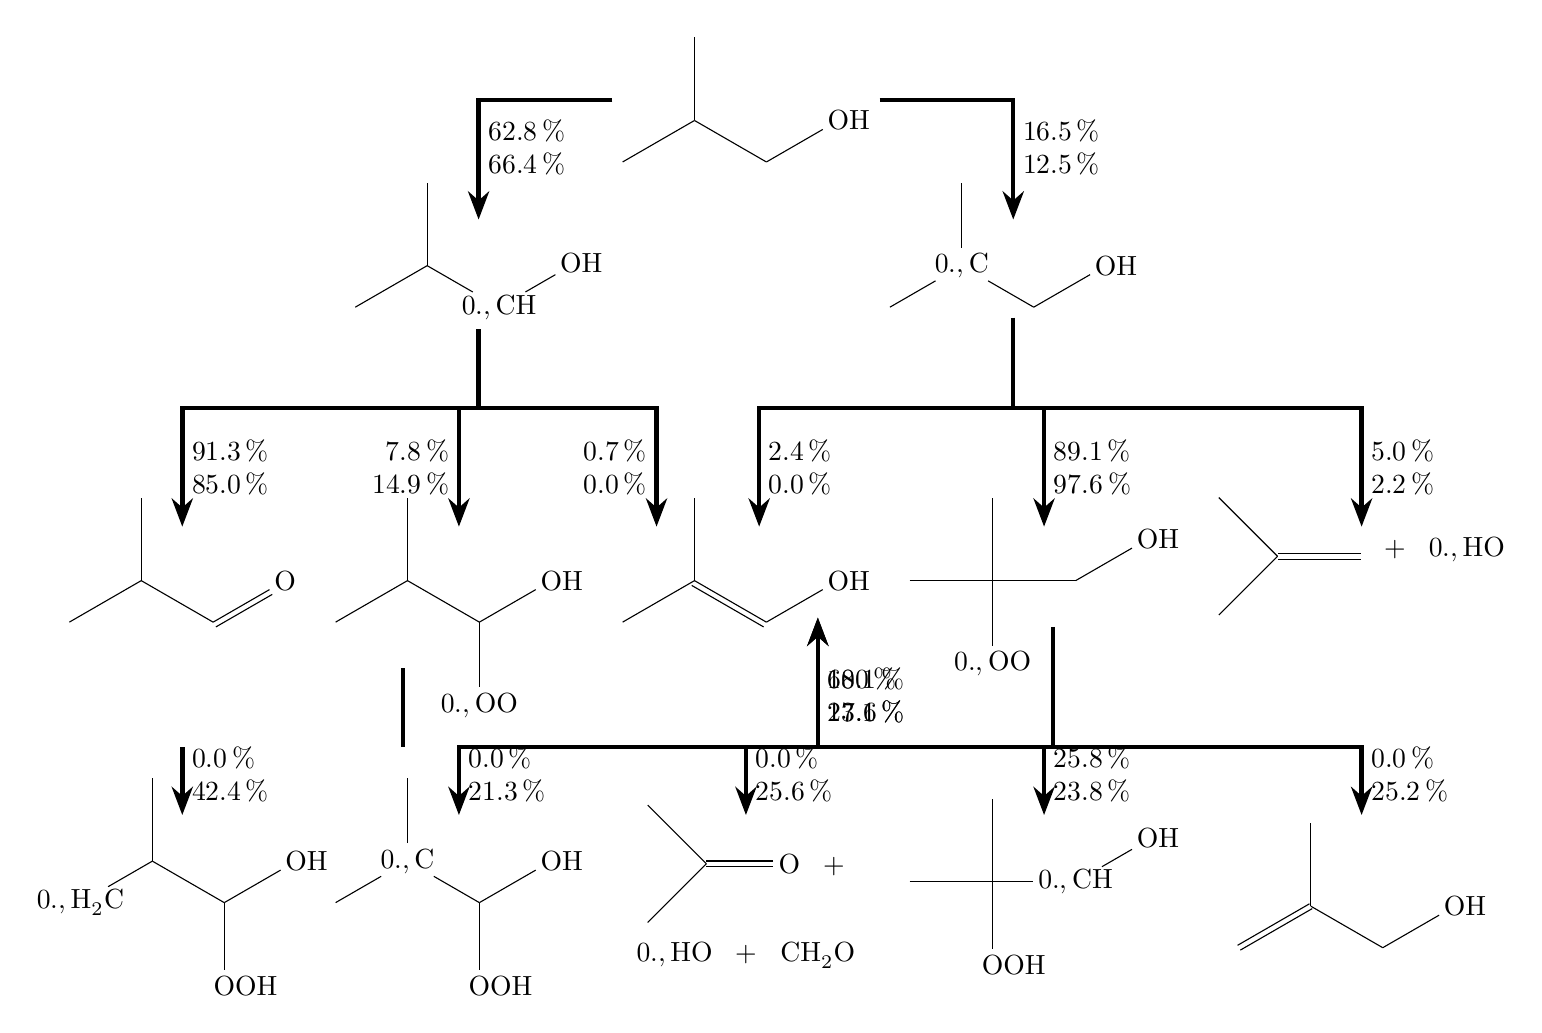
\begin{tikzpicture}[x=1cm, y=1cm, remember picture]
        \begin{scope}
            \node (ibuoh) {\chemfig{-[:30](-[2])-[:330]-[:30]OH}};
            \node[below left=0 and 0 of ibuoh] (aibuoh) {\chemfig{-[:30](-[2])-[:330]\lewis{0.,CH}-[:30]OH}};
            \node[below right=0 and 0 of ibuoh] (bibuoh) {\chemfig{-[:30]\lewis{0.,C}(-[2])-[:330]-[:30]OH}};
            \node[below=4 of ibuoh] (bibuohenol) {\chemfig{-[:30]@{enol-branch}(-[2])=_[:330]-[:30]OH}};
            \node[below=2 of bibuohenol, align=center] (scission) {\chemfig{[:180]O=(-[3])-[5]} \, $+$\\[0.5\baselineskip]\chemfig{\lewis{0.,HO}} \, $+$ \, \ce{CH2O}};
            \node[above left=0 and 0.25 of bibuohenol, anchor=north east] (aibuohoo) {\chemfig{-[:30](-[2])-[:330](-[6]\lewis{0.,OO})-[:30]OH}};
            \path let \p1 = (scission), \p2 = (aibuohoo) in node (aibuohbooh) at (\x2,\y1) {\chemfig{-[:30]\lewis{0.,C}(-[2])-[:330](-[6]OOH)-[:30]OH}};
            \node[above left=0 and 0.25 of aibuohoo, anchor=north east] (ibuohalde) {\chemfig{-[:30]@{alde-branch}(-[2])-[:330]=_[:30]O}};
            \path let \p1 = (scission), \p2 = (ibuohalde) in node (aibuohgooh) at (\x2,\y1) {\chemfig{\lewis{0.,H_2C}-[:30](-[2])-[:330](-[6]OOH)-[:30]OH}};
            \node[above right=0 and 0.25 of bibuohenol, anchor=north west] (bibuohoo) {\chemfig{-(-[2])(-[6]\lewis{0.,OO})--[:30]OH}};
            \path let \p1 = (scission), \p2 = (bibuohoo) in node (bibuohaooh) at (\x2,\y1) {\chemfig{-(-[2])(-[6]OOH)-\lewis{0.,CH}-[:30]OH}};
            \node[above right=0 and 0.25 of bibuohoo, anchor=north west] (isobutene) {\chemfig{[:180]=(-[5])-[3]} \, $+$ \, \chemfig{\lewis{0.,HO}}};
            \path let \p1 = (scission), \p2 = (isobutene) in node (gbutenol) at (\x2,\y1) {\chemfig{=[:30](-[2])-[:330]-[:30]OH}};
        \end{scope}

        \begin{scope}[every path/.style={draw, ultra thick, >={Stealth}}]
            \coordinate (first arrow end) at ($(aibuoh.north)-(0,0.6)$);
            \path[->] (ibuoh.west) -| (first arrow end) coordinate[pos=0.7] (first row);
            \path[->] let \p1 = (ibuoh.east), \p2 = (bibuoh), \p3 = (first arrow end) in (\x1,\y1) -| (\x2,\y3);

            \coordinate (second arrow end) at ($(ibuohalde.north)-(0,0.5)$);
            \coordinate (second row split) at ($(aibuoh.south)-(0,1)$);
            \path let \p1 = (aibuoh.south), \p2 = (second row split) in (\x1,\y1) -- (\x1,\y2);
            \path let \p1 = (bibuoh.south), \p2 = (second row split) in (\x1,\y1) -- (\x1,\y2);
            \path[<->] let \p1 = (second arrow end), \p2 = (second row split), \p3 = (bibuohenol.140), \p4 = (ibuohalde) in (\x4,\y1) -- (\x4,\y2) coordinate[midway] (second row) -- (\x3,\y2) -- (\x3,\y1);
            \path[<->] let \p1 = (second arrow end), \p2 = (second row split), \p3 = (bibuohenol.80), \p4 = (isobutene) in (\x4,\y1) -- (\x4,\y2) -- (\x3,\y2) -- (\x3,\y1);
            \path[->] let \p1 = (aibuohoo), \p2 = (second row split), \p3 = (second arrow end) in (\x1,\y2) -- (\x1,\y3);
            \path[->] let \p1 = (bibuohoo), \p2 = (second row split), \p3 = (second arrow end) in (\x1,\y2) -- (\x1,\y3);

            \coordinate (third arrow end up) at ($(ibuohalde.south)+(0,0.25)$);
            \coordinate (third arrow end dn) at ($(aibuohgooh.north)-(0,0.6)$);
            \coordinate (third row split) at ($(aibuohoo.south)-(0,0.25)$);
            \path let \p1 = ($(aibuohoo.245)+(0,0.75)$), \p2 = (third row split) in (\x1,\y1) -- (\x1,\y2);
            \path let \p1 = ($(bibuohoo.275)+(0,0.75)$), \p2 = (third row split) in (\x1,\y1) -- (\x1,\y2);
            \path[<->] let \p1 = (third arrow end dn), \p2 = (third row split), \p3 = (aibuohbooh), \p4 = (alde-branch), \p5 = (third arrow end up) in (\x4,\y5) -- (\x4,\y2) coordinate[pos=0.6] (third row up) -- (\x3,\y2) -- (\x3,\y1) coordinate[pos=0.4] (third row dn);
            \path[->] let \p1 = (third arrow end dn), \p2 = (aibuohgooh), \p3 = (third row split) in (\x2,\y3) -- (\x2,\y1);
            \path[<->] let \p1 = (enol-branch), \p2 = (third arrow end up), \p3 = (third row split), \p4 = (gbutenol.north), \p5 = (third arrow end dn) in (\x1,\y2) -- (\x1,\y3) -- (\x4,\y3) -- (\x4,\y5);
            \path[->] let \p1 = (scission), \p2 = (third arrow end dn), \p3 = (third row split) in (\x1,\y3) -- (\x1,\y2);
            \path[->] let \p1 = (bibuohaooh), \p2 = (third arrow end dn), \p3 = (third row split) in (\x1,\y3) -- (\x1,\y2);
        \end{scope}

        \path let \p1 = (first row), \p2 = (aibuoh) in node[flux] at (\x2,\y1) {\flux{62.8}{66.4}};
        \path let \p1 = (first row), \p2 = (bibuoh) in node[flux] at (\x2,\y1) {\flux{16.5}{12.5}};
        \path let \p1 = (second row), \p2 = (ibuohalde) in node[flux] at (\x2,\y1) {\flux{91.3}{85.0}};
        \path let \p1 = (second row), \p2 = (aibuohoo) in node[align=right, left] at (\x2,\y1) {\flux{7.8}{14.9}};
        \path let \p1 = (second row), \p2 = (bibuohenol.140) in node[flux, left] at (\x2,\y1) {\flux{0.7}{0.0}};
        \path let \p1 = (second row), \p2 = (bibuohenol.80) in node[flux] at (\x2,\y1) {\flux{2.4}{0.0}};
        \path let \p1 = (second row), \p2 = (bibuohoo) in node[flux] at (\x2,\y1) {\flux{89.1}{97.6}};
        \path let \p1 = (second row), \p2 = (isobutene) in node[flux] at (\x2,\y1) {\flux{5.0}{2.2}};
        \path let \p1 = (third row up), \p2 = (alde-branch) in node[flux] at (\x2,\y1) {\flux{100}{27.6}};
        \path let \p1 = (third row up), \p2 = (enol-branch) in node[flux] at (\x2,\y1) {\flux{68.1}{13.1}};
        \path let \p1 = (third row dn), \p2 = (aibuohgooh) in node[flux] at (\x2,\y1) {\flux{0.0}{42.4}};
        \path let \p1 = (third row dn), \p2 = (aibuohbooh) in node[flux] at (\x2,\y1) {\flux{0.0}{21.3}};
        \path let \p1 = (third row dn), \p2 = (scission) in node[flux] at (\x2,\y1) {\flux{0.0}{25.6}};
        \path let \p1 = (third row dn), \p2 = (bibuohaooh) in node[flux] at (\x2,\y1) {\flux{25.8}{23.8}};
        \path let \p1 = (third row dn), \p2 = (gbutenol) in node[flux] at (\x2,\y1) {\flux{0.0}{25.2}};
    \end{tikzpicture}
\end{document}
